\documentclass[12pt,a4paper]{article}

% ─── Encodage et langue ────────────────────────────────────────
\usepackage[utf8]{inputenc}
\usepackage[T1]{fontenc}
\usepackage[french]{babel}
\usepackage{lmodern} % Police vectorielle pour éviter les bugs

% ─── Mise en page ─────────────────────────────────────────────
\usepackage{geometry}
\geometry{top=2.5cm, bottom=2.5cm, left=3cm, right=3cm}

% ─── Mathématiques ────────────────────────────────────────────
\usepackage{amsmath, amssymb}

% ─── Tableaux ─────────────────────────────────────────────────
\usepackage{booktabs}
\usepackage{array}
\usepackage{multirow}
\usepackage{longtable}
\usepackage{tabularx}

% ─── Graphiques (EN MODE DEMO POUR NE PAS FAIRE PLANTER) ──────
\usepackage{graphicx}
\usepackage{float}
\usepackage{caption}
\usepackage{subcaption}

% ─── Dessin TikZ ──────────────────────────────────────────────
\usepackage{tikz}
\usetikzlibrary{shapes.geometric, arrows.meta, positioning, fit, backgrounds, calc}

% ─── Code source ──────────────────────────────────────────────
\usepackage{listings}
\usepackage{xcolor}

% ─── Mise en forme ────────────────────────────────────────────
\usepackage{fancyhdr}
\usepackage{titlesec}
\usepackage{enumitem}
\usepackage{setspace}
\usepackage{parskip}
\usepackage{hyperref}
\usepackage{mdframed}

% ─── Couleurs (noir et gris uniquement) ───────────────────────
\definecolor{backcolor}{RGB}{245,245,245}
\definecolor{darkgray}{RGB}{60,60,60}
\definecolor{medgray}{RGB}{130,130,130}
\definecolor{lightgray}{RGB}{210,210,210}

\hypersetup{
    colorlinks=true,
    linkcolor=black,
    urlcolor=black,
    citecolor=black,
    pdftitle={Rapport NLP - Détection du Plagiat},
}

% ─── Style code Python ────────────────────────────────────────
\lstdefinestyle{pythonstyle}{
    backgroundcolor=\color{backcolor},
    commentstyle=\color{darkgray}\itshape,
    keywordstyle=\color{black}\bfseries,
    numberstyle=\tiny\color{medgray},
    stringstyle=\color{darkgray},
    basicstyle=\ttfamily\small,
    breaklines=true,
    captionpos=b,
    keepspaces=true,
    numbers=left,
    numbersep=5pt,
    frame=single,
    rulecolor=\color{black},
    xleftmargin=15pt,
    language=Python
}

\lstdefinestyle{bashstyle}{
    backgroundcolor=\color{backcolor},
    basicstyle=\ttfamily\small,
    breaklines=true,
    frame=single,
    rulecolor=\color{black},
    numbers=none,
    xleftmargin=10pt
}

\lstset{style=pythonstyle}

% ─── En-tête / Pied de page ───────────────────────────────────
\pagestyle{fancy}
\fancyhf{}
\fancyhead[L]{\small\textbf{Détection automatique du plagiat}}
\fancyhead[R]{\small\textit{NLP}}
\fancyfoot[C]{\thepage}
\renewcommand{\headrulewidth}{0.5pt}
\renewcommand{\footrulewidth}{0pt}

% ─── Titres  ─────────────────────────────────
\titleformat{\section}
  {\Large\bfseries}{\thesection\quad}{0em}{}[\vspace{2pt}\titlerule\vspace{4pt}]
\titleformat{\subsection}
  {\large\bfseries}{\thesubsection\quad}{0em}{}
\titleformat{\subsubsection}
  {\normalsize\bfseries}{\thesubsubsection\quad}{0em}{}

% ─── Encadré gris ─────────────────────────────────────────────
\newmdenv[
  linecolor=black,
  linewidth=0.8pt,
  innerleftmargin=10pt,
  innerrightmargin=10pt,
  innertopmargin=8pt,
  innerbottommargin=8pt,
  backgroundcolor=backcolor
]{graybox}

\begin{document}
\setstretch{1.15}

% ─── PAGE DE TITRE ────────────────────────────────────────────
\begin{titlepage}
\centering
\vspace*{1cm}

{\LARGE\bfseries Université Caen Normandie}\\[0.3cm]
{\large Unité d'enseignement : Projet 2}\\[0.2cm]
{\large Année universitaire 2025/2026}

\vspace{1cm}
\noindent\rule{\linewidth}{1.5pt}\\[0.5cm]

{\Huge\bfseries Détection Automatique\\[0.3cm] du Plagiat Textuel}\\[0.4cm]

\vspace{0.3cm}
\noindent\rule{\linewidth}{1.5pt}

\vspace{1.5cm}
{\large\bfseries Rapport de Projet}

\vspace{1.5cm}

\begin{tabular}{ll}
\hline\\[2pt]
\textbf{Nom \& Prénom} & \textbf{Rôle principal}\\[4pt]
\hline\\[2pt]
REZGUI Léna                 & k-NN, BoW, BoW n-grams\\[6pt]
Mohamed Chaib Setti         & SVM, TF-IDF, TF-IDF n-grams\\[6pt]
Aris Bensadi                & MLP from scratch, générateur Blob\\[6pt]
LAMAIRI Mohamed Yassine     & Naive Bayes, NER, résultats\\[4pt]
\hline
\end{tabular}

\vspace{2cm}

\begin{tabular}{ll}
\textbf{Corpus}          & PAN Plagiarism Corpus\\[4pt]
\textbf{Tâche}           & Classification 4 classes : \texttt{non}, \texttt{light}, \texttt{heavy}, \texttt{cut}\\[4pt]
\textbf{Classifieurs}    & SVM, $k$-NN, Naive Bayes, MLP (from scratch)\\[4pt]
\textbf{Représentations} & BoW, TF-IDF, N-grammes, NER, Blob synthétique\\
\end{tabular}

\vfill
\end{titlepage}

% ─── TABLE DES MATIÈRES ───────────────────────────────────────
\newpage
\tableofcontents
\newpage


\section{Introduction}

\subsection{Description générale du projet}

Ce projet porte sur la détection automatique du plagiat dans des textes académiques, en appliquant des techniques issues du traitement automatique du langage naturel (TAL) et de l'apprentissage automatique. Concrètement, l'objectif est de prendre un document textuel rédigé par un étudiant et de déterminer automatiquement s'il constitue un plagiat, et si oui, de quel type.

Le plagiat ne se limite pas à la simple copie mot pour mot : il peut prendre des formes subtiles comme la substitution de synonymes, la réécriture de phrases ou la restructuration de paragraphes entiers. Pour détecter ces différentes formes, nous avons choisi une approche par classification supervisée : le système apprend à partir d'exemples étiquetés (des documents dont le niveau de plagiat est connu) à reconnaître les patterns caractéristiques de chaque type de plagiat.

Notre pipeline se décompose en deux grandes étapes. D'abord, les textes bruts sont transformés en représentations numériques (vecteurs de features) via plusieurs méthodes : Bag of Words, TF-IDF, N-grammes, Reconnaissance d'Entités Nommées. Ensuite, ces représentations sont utilisées comme entrées de plusieurs classifieurs : SVM, $k$-NN, Naive Bayes Complémentaire, et un réseau de neurones MLP implémenté entièrement à la main en NumPy.

\subsection{Présentation du plan du rapport}

Ce rapport est organisé en sept sections. La section~2 présente les objectifs du projet, la problématique, et un tour d'horizon des travaux existants. La section~3 décrit les fonctionnalités implémentées et la répartition des tâches au sein du groupe. La section~4 détaille les éléments techniques : algorithmes, structures de données et description du corpus. La section~5 présente l'architecture logicielle du projet, les bibliothèques utilisées et les interactions entre modules. La section~6 expose les expérimentations conduites et les résultats obtenus avec les graphiques issus de nos expériences. Enfin, la section~7 conclut le rapport et propose des pistes d'amélioration.

\section{Objectifs du projet}

\subsection{Problématique}

La question centrale de ce projet est la suivante : \textit{est-il possible, à partir du seul contenu textuel d'un document, de déterminer automatiquement s'il a été plagié et de quelle façon ?}

La difficulté principale réside dans la diversité des formes de plagiat. Un copier-coller direct est trivial à détecter par comparaison de chaînes de caractères. En revanche, un texte fortement paraphrasé, dans lequel les idées et la structure sont conservées mais le vocabulaire est presque entièrement remplacé par des synonymes, est beaucoup plus difficile à identifier. Les méthodes lexicales classiques (comparaison de mots) sont insuffisantes pour ce cas, et l'on touche ici aux limites des approches purement statistiques sur le texte brut.
Par ailleurs, dans un contexte académique réel, un système de détection de plagiat doit être capable de traiter des documents qui n'ont jamais été vus à l'entraînement, avec un minimum de faux positifs (accuser un étudiant innocent) et un minimum de faux négatifs (manquer un cas de plagiat réel).

\subsection{Points-clés et grandes étapes}

Le projet s'articule autour de cinq grandes étapes :

\begin{enumerate}[leftmargin=1.5cm]
    \item \textbf{Prétraitement et exploration des données} : analyse du corpus PAN, compréhension de la taxonomie des classes, identification du déséquilibre entre classes.

    \item \textbf{Représentation vectorielle des textes} : implémentation de six méthodes de vectorisation (BoW, TF-IDF, BoW+Ngrams, TF-IDF+Ngrams, NER+BoW, Blob synthétique). Chaque méthode produit un fichier CSV consommé par les classifieurs.

    \item \textbf{Implémentation des classifieurs} : développement de quatre classifieurs avec leurs boucles d'hyperparamètres (SVM, $k$-NN, Naive Bayes Complémentaire, MLP from scratch).

    \item \textbf{Évaluation et comparaison} : calcul des métriques (accuracy, F1-score macro, recall macro) pour toutes les combinaisons représentation/classifieur/hyperparamètre, soit 84 configurations au total.

    \item \textbf{Analyse des résultats} : identification des meilleures configurations, analyse des erreurs par classe, discussion des limites et des pistes d'amélioration.
\end{enumerate}

\subsection{Méthodologie et défis liés aux données}

Notre approche repose sur un pipeline de traitement séquentiel strict. Dans un premier temps, les textes bruts passent par des algorithmes de \textbf{représentation vectorielle} afin d'être transformés en tenseurs numériques. Ensuite, ces données sont passées à nos \textbf{classifieurs} qui apprennent à identifier la classe de plagiat correspondante.

Cependant, le corpus PAN utilisé pour ce projet présente deux défis majeurs en apprentissage automatique :
\begin{itemize}
    \item \textbf{Taille réduite} : Le jeu de données ne contient que 95 documents au total. Entraîner des modèles, particulièrement un réseau de neurones MLP, sur si peu d'exemples augmente drastiquement le risque de sur-apprentissage (\textit{overfitting}).
    \item \textbf{Déséquilibre des classes (Imbalanced data)} : La distribution des exemples n'est pas uniforme. La classe majoritaire \texttt{non} (aucun plagiat) représente 40\,\% du corpus, tandis que les classes \texttt{light}, \texttt{heavy} et \texttt{cut} n'en représentent que 20\,\% chacune.
\end{itemize}

Pour corriger ce déséquilibre et garantir une évaluation rigoureuse, nous avons intégré deux mécanismes clés dans notre développement :

\begin{description}[style=nextline, leftmargin=1.5cm]
    \item[Échantillonnage stratifié (\texttt{stratify})]
    Lors de la division du corpus en ensembles d'entraînement et de test (split 70/30), nous utilisons l'option de stratification. Cela force l'algorithme à maintenir exactement la même proportion de chaque classe dans l'ensemble de test que dans l'ensemble global. Sans cela, un tirage aléatoire risquerait de placer tous les documents d'une classe minoritaire dans le même ensemble, faussant totalement l'apprentissage.

    \item[Pondération des classes (\texttt{class\_weight})]
    Pour empêcher nos algorithmes de «~tricher~» en prédisant systématiquement la classe majoritaire \texttt{non}, nous appliquons des poids inversement proportionnels aux fréquences des classes (par exemple \texttt{class\_weight='balanced'} pour le SVM). Ainsi, lorsqu'un classifieur se trompe sur une classe minoritaire comme \texttt{light}, l'erreur est pénalisée beaucoup plus fortement lors de la mise à jour de ses paramètres. Le Naive Bayes Complémentaire a également été spécifiquement choisi car sa formulation mathématique est naturellement robuste face aux données déséquilibrées.
\end{description}

\section{Fonctionnalités implémentées}

\subsection{Description des fonctionnalités}

Le projet propose un pipeline complet et modulaire de détection du plagiat. Les fonctionnalités suivantes ont été implémentées :

\begin{description}[style=nextline, leftmargin=1.5cm]
    \item[Génération de représentations vectorielles]
    À partir des textes bruts du corpus, six représentations numériques sont générées automatiquement et sauvegardées au format CSV dans le dossier \texttt{data/}. Ces représentations capturent différents niveaux d'information linguistique.

    \item[Classification multi-classe]
    Quatre classifieurs sont disponibles, chacun capable de prédire l'une des quatre classes de plagiat (\texttt{non}, \texttt{light}, \texttt{heavy}, \texttt{cut}) pour n'importe quel document vectorisé.

    \item[Recherche d'hyperparamètres]
    Chaque classifieur effectue automatiquement une boucle sur plusieurs valeurs d'hyperparamètres et produit un fichier de résultats par configuration.

    \item[Fusion des résultats multi-représentations]
    Pour une même configuration d'hyperparamètre, les prédictions de toutes les représentations sont fusionnées dans un unique fichier CSV permettant la comparaison directe.

    \item[Génération automatique de graphiques]
    Le script \texttt{results.py} lit tous les fichiers de résultats et génère des graphiques en barres du Top-6 des meilleures configurations, triées par F1-score macro.

    \item[Exécution en un seul appel]
    Le script \texttt{run\_pipeline.sh} orchestre l'ensemble du pipeline en une seule commande shell.

    \item[Jeu de données synthétique (Blob)]
    Un générateur de données synthétiques (\texttt{blob.py}) produit 80 exemples artificiels à classes parfaitement séparables, permettant de valider le bon fonctionnement des classifieurs.
\end{description}

\subsection{Organisation du projet --- Qui a fait quoi}

\begin{table}[H]
\centering
\caption{Répartition des tâches entre les membres du groupe}
\label{tab:repartition}
\begin{tabularx}{\textwidth}{lX}
\toprule
\textbf{Membre} & \textbf{Contributions} \\
\midrule
\textbf{REZGUI Léna}
& Implémentation du classifieur $k$-NN (\texttt{knn.py}) avec distance cosinus. Implémentation des représentations vectorielles : \texttt{bow.py} (Bag of Words) et \texttt{bow\_ngrams.py} (bigrammes). Analyse exploratoire du corpus PAN et mise en place de la structure des fichiers CSV. \\
\addlinespace
\textbf{SETTI Mohamed Chaib}
& Implémentation du classifieur SVM (\texttt{svm\_.py}) avec noyau cosinus précalculé et gestion du paramètre $C$. Implémentation de \texttt{tf\_idf.py} (TF-IDF unigrams) et \texttt{tf\_idf\_ngram.py} (trigrammes). Gestion du split de référence partagé entre classifieurs. \\
\addlinespace
\textbf{BENSADI Aris}
& Implémentation complète du réseau de neurones MLP \textit{from scratch} en NumPy (\texttt{mlp.py}) : couches denses, ReLU, Softmax, optimiseur Adam, cross-entropie, backpropagation. Développement du générateur synthétique \texttt{blob.py}. Rédaction du script d'orchestration \texttt{run\_pipeline.sh}. \\
\addlinespace
\textbf{LAMAIRI Mohamed Yassine}
& Implémentation du classifieur Naive Bayes Complémentaire (\texttt{naivebayes.py}) avec boucle sur alpha. Développement de la représentation NER+BoW (\texttt{ner.py}) avec spaCy. Implémentation du module de visualisation \texttt{results.py} et validation des sorties CSV. \\
\bottomrule
\end{tabularx}
\end{table}

\section{Éléments techniques}

\subsection{Méthodes de représentation textuelle}

\subsubsection{Bag of Words (BoW) et N-grammes (\texttt{bow.py}, \texttt{bow\_ngrams.py})}
L'approche Bag of Words transforme les textes en vecteurs représentant la fréquence d'apparition de chaque mot, via le \texttt{CountVectorizer} de scikit-learn. Afin de capturer un contexte plus riche que de simples mots isolés, l'extension aux N-grammes (ici des bigrammes) permet d'extraire et de compter des paires de mots adjacents. Cela s'avère crucial pour détecter le plagiat de type \texttt{cut}, où des séquences exactes sont copiées du texte source.

\subsubsection{TF-IDF et N-grammes (\texttt{tf\_idf.py}, \texttt{tf\_idf\_ngram.py})}
La pondération TF-IDF (\textit{Term Frequency-Inverse Document Frequency}) associe à chaque terme $t$ dans un document $d$ un score défini par :
$$
\text{TF-IDF}(t,d) = \underbrace{\frac{\text{freq}(t,d)}{|d|}}_{\text{TF}} \times \underbrace{\log\frac{N}{1+\text{df}(t)}}_{\text{IDF}}
$$
où $N$ est le nombre de documents et $\text{df}(t)$ le nombre de documents contenant le terme $t$. Associée aux n-grammes (allant jusqu'aux trigrammes dans notre pipeline), cette méthode pondère plus lourdement les expressions discriminantes et spécifiques tout en pénalisant les termes trop fréquents du corpus.

\subsubsection{Reconnaissance d'Entités Nommées (\texttt{ner.py})}
Pour cette représentation vectorielle, nous utilisons la bibliothèque \texttt{spaCy} (\texttt{en\_core\_web\_sm}) pour extraire préalablement toutes les entités nommées (personnes, dates, lieux, organisations) présentes dans un document. Les espaces entre les mots de ces entités sont remplacés par des tirets bas, et l'ensemble est passé au \texttt{CountVectorizer} pour générer un «~Bag of Entities~». L'objectif est de détecter un plagiat lourd via la structure factuelle, indépendamment de la paraphrase.

\subsubsection{Générateur de données synthétiques Blob (\texttt{blob.py})}
Afin de valider théoriquement et unitairement le bon fonctionnement de tous nos classifieurs, un jeu de données artificiel est généré. Il crée 80 documents (20 par classe) et leur attribue des fréquences précises pour trois variables factices (\texttt{mot\_original}, \texttt{mot\_copie}, \texttt{mot\_synonyme}) de manière à créer des signatures de données parfaitement séparables pour chaque niveau de plagiat.

\subsection{Algorithmes de classification}

\subsubsection{SVM avec noyau cosinus précalculé (\texttt{svm\_.py})}
Le classifieur SVM (\textit{Support Vector Machine}) cherche l'hyperplan de marge maximale séparant les classes. Sa formulation primale est :
$$
\min_{\mathbf{w}, b, \xi} \frac{1}{2}\|\mathbf{w}\|^2 + C \sum_{i=1}^n \xi_i
\quad \text{s.t.} \quad y_i\bigl(\mathbf{w}^\top \phi(x_i) + b\bigr) \geq 1 - \xi_i,\quad \xi_i \geq 0
$$
où $C$ contrôle le compromis biais-variance. La particularité technique de notre implémentation est l'utilisation d'un \textbf{noyau cosinus précalculé}. Plutôt que de passer les features brutes de nos matrices (parfois très larges), on calcule d'abord la matrice de Gram $K$ via \texttt{cosine\_similarity} :
$$
K_{ij} = \frac{\mathbf{x}_i \cdot \mathbf{x}_j}{\|\mathbf{x}_i\| \cdot \|\mathbf{x}_j\|}
$$
Cette mesure d'angle entre les vecteurs neutralise les effets dus à la longueur inégale des documents.

\subsubsection{Réseau de neurones MLP from scratch (\texttt{mlp.py})}
Le MLP a été codé intégralement en utilisant NumPy :
\begin{itemize}
    \item \textbf{Initialisation de Glorot (Xavier) :} $W \sim \mathcal{U}\!\left(-\sqrt{\frac{6}{n_{\mathrm{in}} + n_{\mathrm{out}}}},\ +\sqrt{\frac{6}{n_{\mathrm{in}} + n_{\mathrm{out}}}}\right)$ pour éviter l'explosion des gradients.
    \item \textbf{Softmax numériquement stable :} $\sigma(\mathbf{z})_i = \frac{e^{z_i - \max(\mathbf{z})}}{\sum_j e^{z_j - \max(\mathbf{z})}}$ pour se prémunir contre les dépassements de capacité (\textit{overflow}).
    \item \textbf{Optimiseur Adam :} Utilisation des moments pour la backpropagation avec $\beta_1=0.9$, $\beta_2=0.999$, $\epsilon=10^{-8}$. La fonction de perte exploitée est l'entropie croisée (Cross-Entropy).
\end{itemize}

\subsubsection{Naive Bayes Complémentaire (\texttt{naivebayes.py})}
La variante Complémentaire du Naive Bayes (CNB) est particulièrement adaptée aux jeux de données déséquilibrés. Contrairement à la variante standard qui estime la probabilité d'un terme étant donnée une classe, le CNB estime $P(t \mid \bar{c})$, soit la probabilité d'un terme dans toutes les autres classes.
$$
\hat{y} = \arg\min_{c} \sum_{t} \text{freq}(t, d) \cdot \log P(t \mid \bar{c})
$$
Cela évite aux classes majoritaires (ici la classe \texttt{non}) d'écraser les prédictions.

\subsubsection{$k$-Plus Proches Voisins (\texttt{knn.py})}
L'algorithme des $k$-NN vérifie pour chaque document suspect les $k$ documents les plus proches dans l'espace d'entraînement. Afin d'être pertinent face aux variations des textes, le classifieur \texttt{KNeighborsClassifier} a été explicitement configuré avec la \texttt{metric='cosine'} au lieu de la distance euclidienne par défaut.

\subsection{Structures de données non triviales}

\subsubsection{Matrice de Gram pour le SVM}
Le SVM avec noyau précalculé exige une structure particulière. À l'entraînement, la matrice passée est la sous-matrice carrée $K[\text{train},:][:,\text{train}]$. Au test, la matrice est $K[\text{test},:][:,\text{train}]$ (lignes = exemples de test, colonnes = exemples d'entraînement). Cette asymétrie est gérée explicitement dans le script.

\subsubsection{Split de référence partagé}
Pour garantir la comparabilité des résultats entre toutes les représentations, un \textbf{split de référence unique} est défini une fois sur le premier CSV chargé (\texttt{random\_state=42, stratify=Category}) et réutilisé pour tous les CSV de même taille. Les CSV de taille différente (Blob, 80 exemples vs. 95) font l'objet d'un split indépendant.

\subsubsection{Classe Layer et accumulation des gradients}
Dans \texttt{mlp.py}, la classe \texttt{Layer} encapsule poids, biais, gradients accumulés et optimiseur Adam propre à la couche. Les gradients sont accumulés sur tout le batch (\texttt{batch\_counter} trace le nombre d'exemples vus) avant d'appliquer la mise à jour Adam, ce qui est équivalent à un mini-batch gradient descent.

\subsection{Description des données}

\subsubsection{Corpus PAN}
Le corpus est issu des compétitions PAN dédiées à la détection du plagiat. Il contient des paires document suspect / document source, organisées par tâches.

\begin{table}[H]
\centering
\caption{Distribution des classes dans le corpus (95 documents effectifs)}
\label{tab:corpus}
\begin{tabular}{lccl}
\toprule
\textbf{Classe} & \textbf{Effectif} & \textbf{\%} & \textbf{Description} \\
\midrule
\texttt{non}   & 38 & 40,0 & Aucun plagiat --- texte entièrement original \\
\texttt{cut}   & 19 & 20,0 & Copier-coller direct sans modification \\
\texttt{heavy} & 19 & 20,0 & Paraphrase forte, restructuration syntaxique \\
\texttt{light} & 19 & 20,0 & Substitution de synonymes, réécriture partielle \\
\midrule
\texttt{orig}  & 5  & exclu & Textes sources (non utilisés en classification) \\
\midrule
\textbf{Total} & \textbf{95} & \textbf{100} & \\
\bottomrule
\end{tabular}
\end{table}

\subsubsection{Format des CSV de représentation}
Chaque méthode de représentation produit un fichier CSV dont les colonnes \texttt{File}, \texttt{Task}, \texttt{Category} contiennent les métadonnées, suivies par les features numériques.

\begin{table}[H]
\centering
\caption{Taille approximative des matrices de représentation}
\label{tab:matrices}
\begin{tabular}{lcc}
\toprule
\textbf{Représentation} & \textbf{Lignes} & \textbf{Colonnes (features)} \\
\midrule
BoW                & 95 & $\sim$4\,300 \\
TF-IDF             & 95 & $\sim$4\,000 \\
BoW + bigrammes    & 95 & $\sim$18\,700 \\
TF-IDF + trigrammes & 95 & $\sim$21\,500 \\
NER + BoW          & 95 & $\sim$620 \\
Blob synthétique   & 80 & 3 \\
\bottomrule
\end{tabular}
\end{table}

\section{Architecture du projet}

\subsection{Paquetages non standards utilisés}

\begin{table}[H]
\centering
\caption{Bibliothèques Python tierces utilisées dans le projet}
\label{tab:packages}
\begin{tabular}{lll}
\toprule
\textbf{Bibliothèque} & \textbf{Version min.} & \textbf{Usage} \\
\midrule
\texttt{scikit-learn} & 1.0 & SVM, $k$-NN, CNB, vectoriseurs, métriques \\
\texttt{numpy}        & 1.21 & Calculs matriciels, MLP from scratch, Adam \\
\texttt{pandas}       & 1.3  & Lecture/écriture CSV, DataFrames \\
\texttt{spacy}        & 3.0  & Extraction d'entités nommées (NER) \\
\texttt{matplotlib}   & 3.4  & Génération des graphiques de résultats \\
\bottomrule
\end{tabular}
\end{table}

\subsection{Diagramme des modules}

\begin{figure}[H]
\centering
\resizebox{\textwidth}{!}{
\begin{tikzpicture}[
    node distance=1.0cm and 1.8cm,
    box/.style={draw=black, thick, rounded corners=3pt, minimum width=3.2cm,
                minimum height=0.75cm, align=center, font=\small\ttfamily,
                fill=backcolor},
    bigbox/.style={draw=black, very thick, rounded corners=4pt,
                   minimum width=3.4cm, minimum height=1.1cm,
                   align=center, font=\small\bfseries, fill=lightgray},
    arr/.style={-{Stealth[length=5pt]}, thick, black}
]

% Colonne 1 : raw_texts
\node[bigbox] (raw) at (0,0) {\texttt{raw\_texts/}\\fichiers .txt};

% Colonne 2 : representation
\node[box] (bow)   at (4.5, 2.5)  {\texttt{bow.py}};
\node[box] (tfidf) at (4.5, 1.5)  {\texttt{tf\_idf.py}};
\node[box] (bgram) at (4.5, 0.5)  {\texttt{bow\_ngrams.py}};
\node[box] (tgram) at (4.5,-0.5)  {\texttt{tf\_idf\_ngram.py}};
\node[box] (ner)   at (4.5,-1.5)  {\texttt{ner.py}};
\node[box] (blob)  at (4.5,-2.5)  {\texttt{blob.py}};

% Colonne 3 : data/
\node[bigbox] (data) at (9.0, 0)   {\texttt{data/}\\CSV vectorisés};

% Colonne 4 : classifiers
\node[box] (svm) at (13.5, 1.5) {\texttt{svm\_.py}};
\node[box] (knn) at (13.5, 0.5) {\texttt{knn.py}};
\node[box] (nb)  at (13.5,-0.5) {\texttt{naivebayes.py}};
\node[box] (mlp) at (13.5,-1.5) {\texttt{mlp.py}};

% Colonne 5 : resultats/
\node[bigbox] (res) at (18.0, 0) {\texttt{resultats/}\\CSV + PNG};

% Flèches raw -> representations
\foreach \rep in {bow, tfidf, bgram, tgram, ner, blob}
    \draw[arr] (raw.east) -- (\rep.west);

% Flèches representations -> data
\foreach \rep in {bow, tfidf, bgram, tgram, ner, blob}
    \draw[arr] (\rep.east) -- (data.west);

% Flèches data -> classifiers
\foreach \clf in {svm, knn, nb, mlp}
    \draw[arr] (data.east) -- (\clf.west);

% Flèches classifiers -> resultats
\foreach \clf in {svm, knn, nb, mlp}
    \draw[arr] (\clf.east) -- (res.west);

\end{tikzpicture}

}
\caption{Diagramme des modules : flux de données du pipeline de gauche à droite}
\label{fig:modules}
\end{figure}

\subsection{Chaînes de traitement}

\subsubsection{Phase 1 --- De texte brut à vecteur numérique}

Chaque script de représentation suit la même chaîne de traitement :

\begin{enumerate}
    \item Lecture de \texttt{file\_information.csv} pour obtenir la liste des fichiers et leurs labels.
    \item Exclusion des documents sources (\texttt{Category='orig'}).
    \item Lecture du contenu texte de chaque fichier \texttt{.txt} dans \texttt{raw\_texts/}.
    \item Vectorisation via l'outil approprié (CountVectorizer, TfidfVectorizer, ou spaCy pour NER).
    \item Concaténation des métadonnées (\texttt{File, Task, Category}) et de la matrice de features.
    \item Écriture du CSV résultant dans \texttt{data/}.
\end{enumerate}

\subsubsection{Phase 2 --- Classification et évaluation}

Chaque classifieur suit la même logique :

\begin{enumerate}
    \item Lecture de tous les CSV passés en argument depuis \texttt{data/}.
    \item Définition du split 70/30 stratifié sur le premier CSV (\texttt{random\_state=42}).
    \item Pour chaque valeur d'hyperparamètre et chaque CSV : entraînement, prédiction, calcul de l'accuracy.
    \item Fusion des prédictions de toutes les représentations dans un CSV groupé par valeur d'hyperparamètre.
    \item Sauvegarde dans \texttt{resultats/} sous la convention \texttt{\{MODELE\}\_results\_\{PARAM\}.csv}.
\end{enumerate}

\subsubsection{Phase 3 --- Visualisation des résultats}

\texttt{results.py} charge tous les CSV de résultats, calcule le F1-score macro et le recall macro, trie toutes les configurations par F1 décroissant, et génère des graphiques en barres (Top-6 par modèle, Top-6 global).

\section{Expérimentations}

\subsection{Exemple d'utilisation --- Exécution du pipeline}

L'ensemble du pipeline s'exécute en une seule commande depuis la racine du projet :

\begin{lstlisting}[style=bashstyle, caption={Lancement complet du pipeline}]
$ chmod +x run_pipeline.sh
$ ./run_pipeline.sh
\end{lstlisting}

\subsection{Résultats quantifiables}

\subsubsection{Résultats SVM}

\begin{figure}[H]
    \centering
    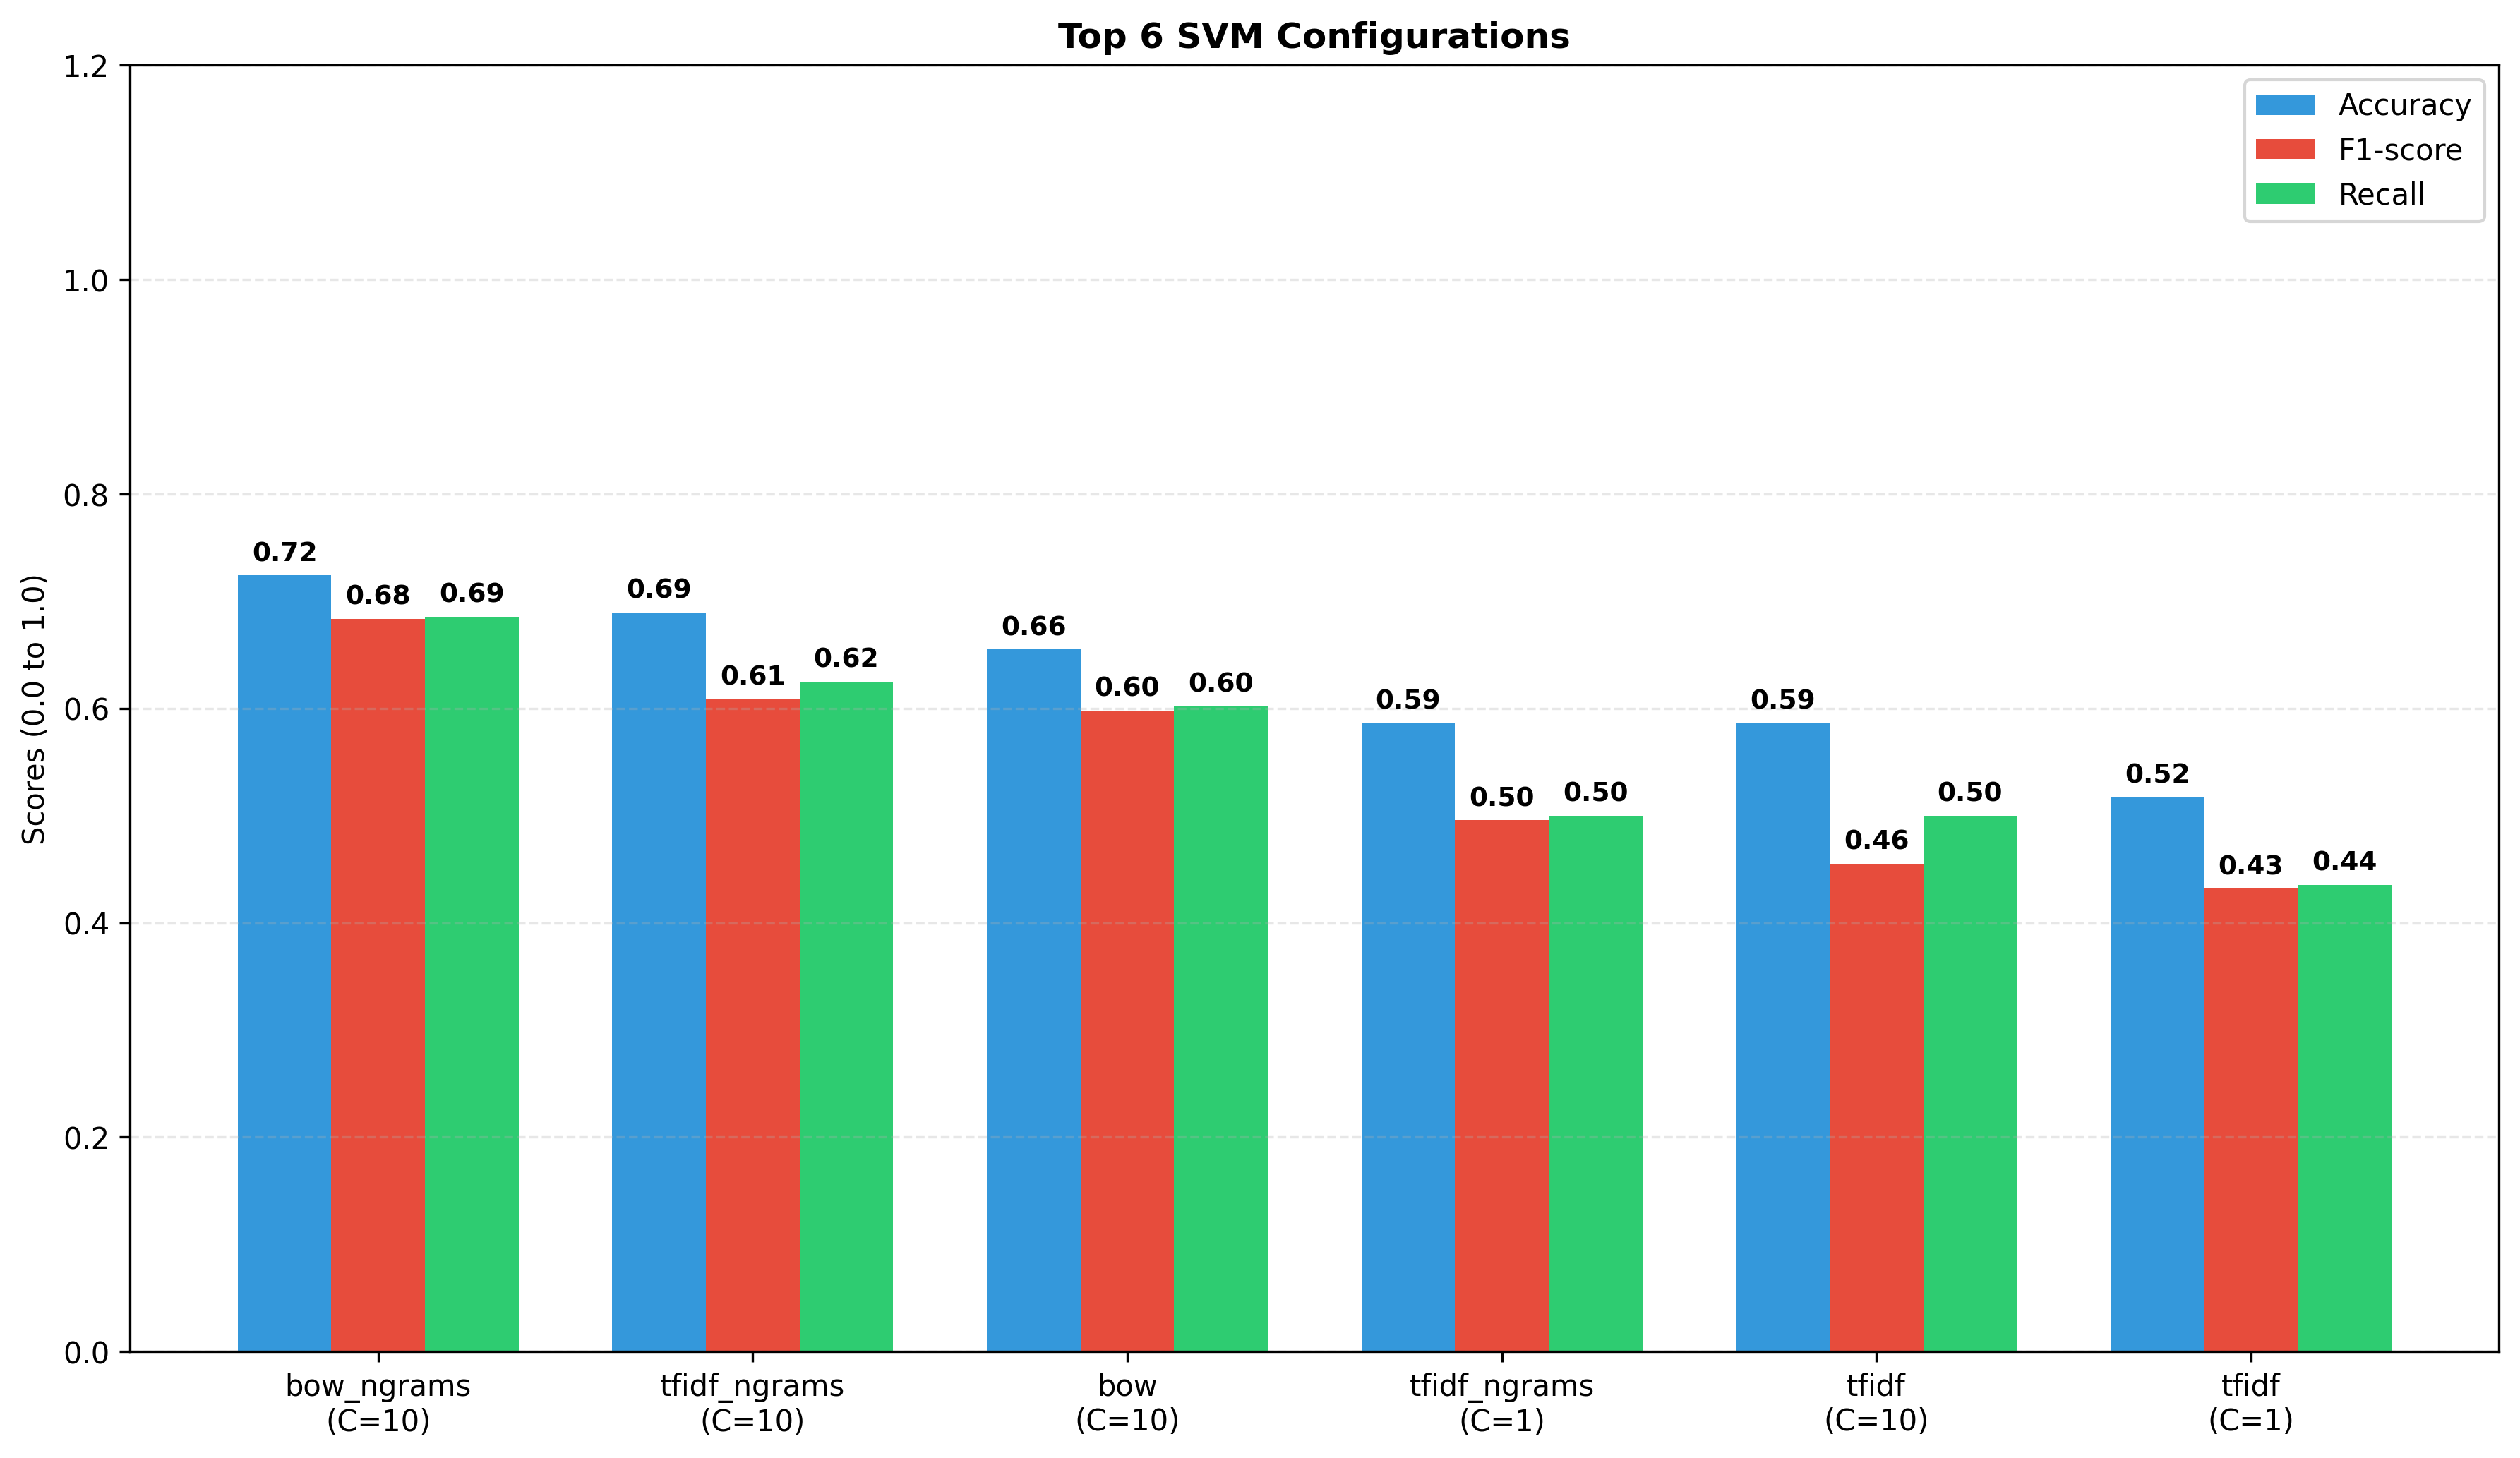
\includegraphics[width=\textwidth]{Top_6_SVM_Configurations.png}
    \caption{Top 6 configurations SVM (triées par F1-score macro décroissant)}
    \label{fig:svm}
\end{figure}

La Figure~\ref{fig:svm} montre les six meilleures configurations SVM. La meilleure est \textbf{TF-IDF N-grammes avec $C=10$} : accuracy \textbf{0,69}, F1-score \textbf{0,61}, recall \textbf{0,62}.

\begin{table}[H]
\centering
\caption{Résultats numériques SVM --- Top 6}
\label{tab:svm_res}
\begin{tabular}{llccc}
\toprule
\textbf{Représentation} & \textbf{$C$} & \textbf{Accuracy} & \textbf{F1-score} & \textbf{Recall} \\
\midrule
tfidf\_ngrams & 10  & 0,69 & 0,61 & 0,62 \\
tfidf\_ngrams & 1   & 0,59 & 0,50 & 0,50 \\
tfidf         & 10  & 0,59 & 0,46 & 0,50 \\
tfidf         & 1   & 0,52 & 0,43 & 0,44 \\
tfidf\_ngrams & 0,1 & 0,38 & 0,14 & 0,25 \\
tfidf         & 0,1 & 0,38 & 0,14 & 0,25 \\
\bottomrule
\end{tabular}
\end{table}

\subsubsection{Résultats $k$-NN}

\begin{figure}[H]
    \centering
    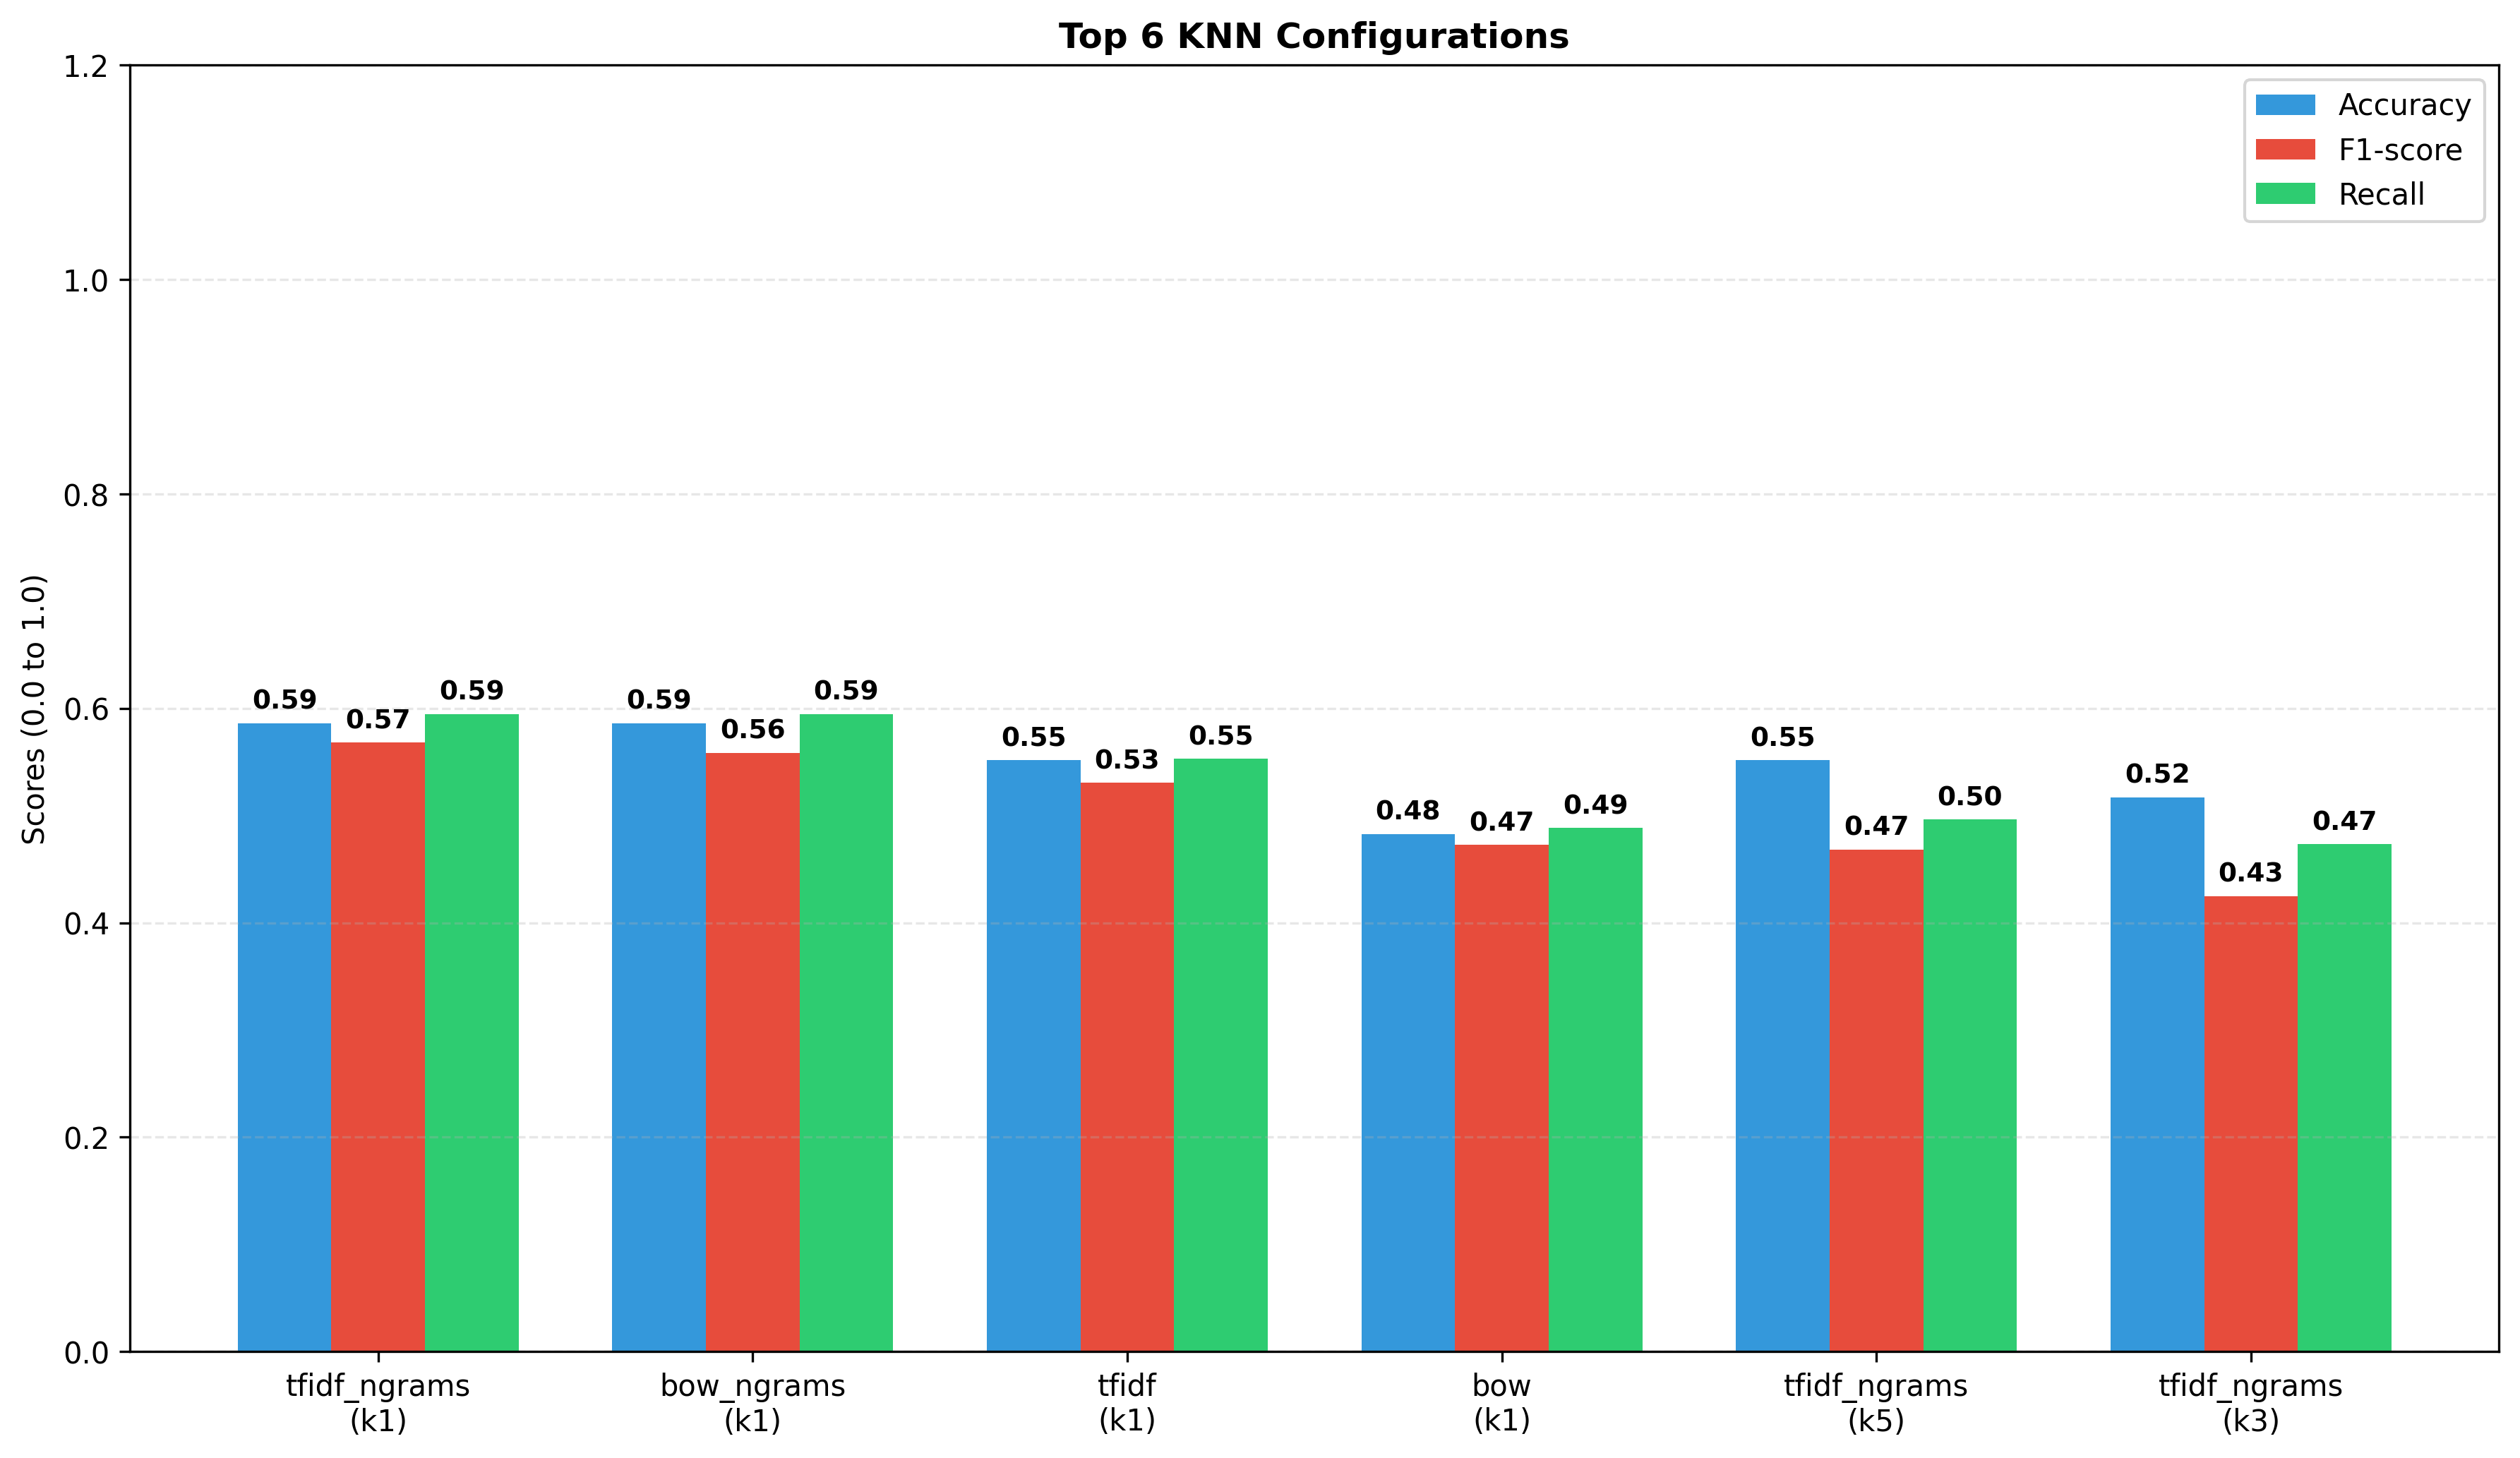
\includegraphics[width=\textwidth]{Top_6_KNN_Configurations.png}
    \caption{Top 6 configurations $k$-NN (triées par F1-score macro décroissant)}
    \label{fig:knn}
\end{figure}

La Figure~\ref{fig:knn} montre les six meilleures configurations $k$-NN. Les deux premières configurations (TF-IDF N-grammes $k=1$ et BoW N-grammes $k=1$) atteignent toutes deux une accuracy de \textbf{0,59} avec des F1-scores de \textbf{0,57} et \textbf{0,56} respectivement.

\begin{table}[H]
\centering
\caption{Résultats numériques $k$-NN --- Top 6}
\label{tab:knn_res}
\begin{tabular}{llccc}
\toprule
\textbf{Représentation} & \textbf{$k$} & \textbf{Accuracy} & \textbf{F1-score} & \textbf{Recall} \\
\midrule
tfidf\_ngrams & 1 & 0,59 & 0,57 & 0,59 \\
bow\_ngrams   & 1 & 0,59 & 0,56 & 0,59 \\
tfidf         & 1 & 0,55 & 0,53 & 0,55 \\
bow           & 1 & 0,48 & 0,47 & 0,49 \\
tfidf\_ngrams & 5 & 0,55 & 0,47 & 0,50 \\
tfidf\_ngrams & 3 & 0,52 & 0,43 & 0,47 \\
\bottomrule
\end{tabular}
\end{table}

\subsubsection{Résultats Naive Bayes}

\begin{figure}[H]
    \centering
    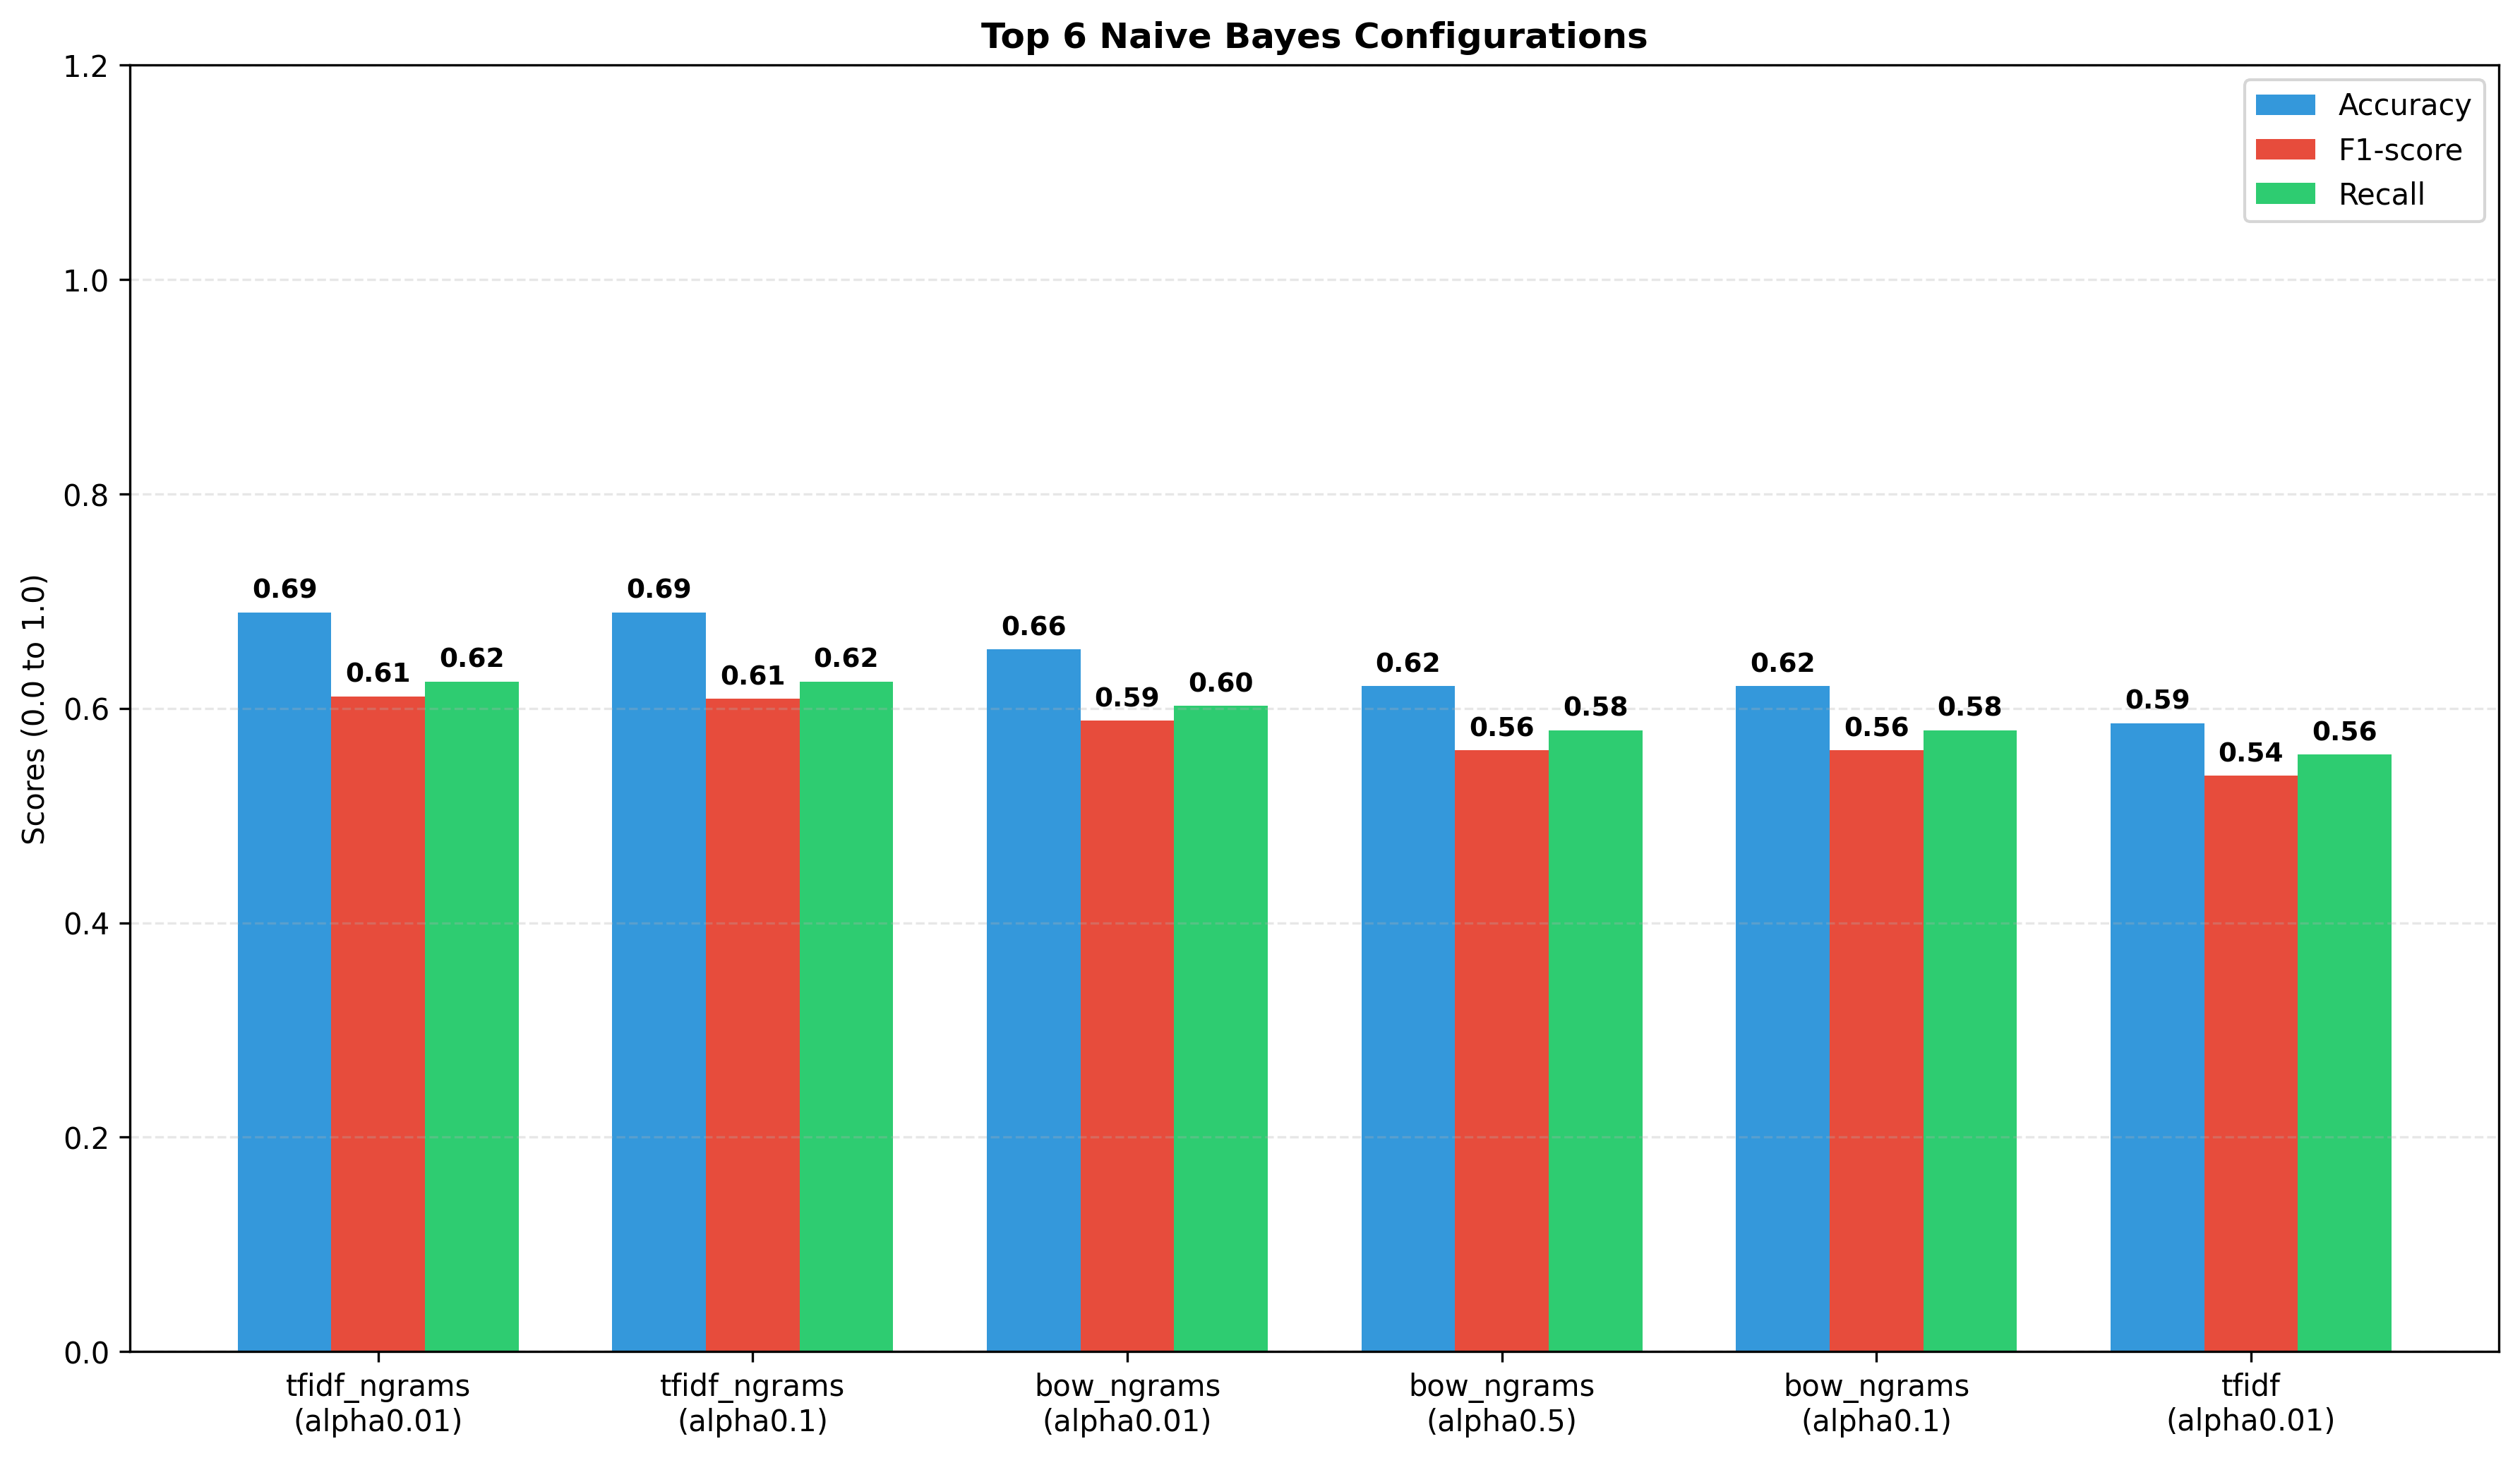
\includegraphics[width=\textwidth]{Top_6_Naive_Bayes_Configurations.png}
    \caption{Top 6 configurations Naive Bayes (triées par F1-score macro décroissant)}
    \label{fig:nb}
\end{figure}

La Figure~\ref{fig:nb} montre les six meilleures configurations pour le classifieur Naive Bayes Complémentaire. Les représentations \textbf{TF-IDF N-grammes} avec $\alpha=0{,}01$ et $\alpha=0{,}1$ dominent avec une accuracy de \textbf{0,69} et un F1-score de \textbf{0,61}, égalant ainsi les performances de pointe obtenues par le SVM.

\begin{table}[H]
\centering
\caption{Résultats numériques Naive Bayes --- Top 6}
\label{tab:nb_res}
\begin{tabular}{llccc}
\toprule
\textbf{Représentation} & \textbf{$\alpha$} & \textbf{Accuracy} & \textbf{F1-score} & \textbf{Recall} \\
\midrule
tfidf\_ngrams & 0,01 & 0,69 & 0,61 & 0,62 \\
tfidf\_ngrams & 0,1  & 0,69 & 0,61 & 0,62 \\
bow\_ngrams   & 0,01 & 0,66 & 0,59 & 0,60 \\
bow\_ngrams   & 0,5  & 0,62 & 0,56 & 0,58 \\
bow\_ngrams   & 0,1  & 0,62 & 0,56 & 0,58 \\
tfidf         & 0,01 & 0,59 & 0,54 & 0,56 \\
\bottomrule
\end{tabular}
\end{table}

\subsubsection{Résultats globaux --- Toutes configurations confondues}

\begin{figure}[H]
    \centering
    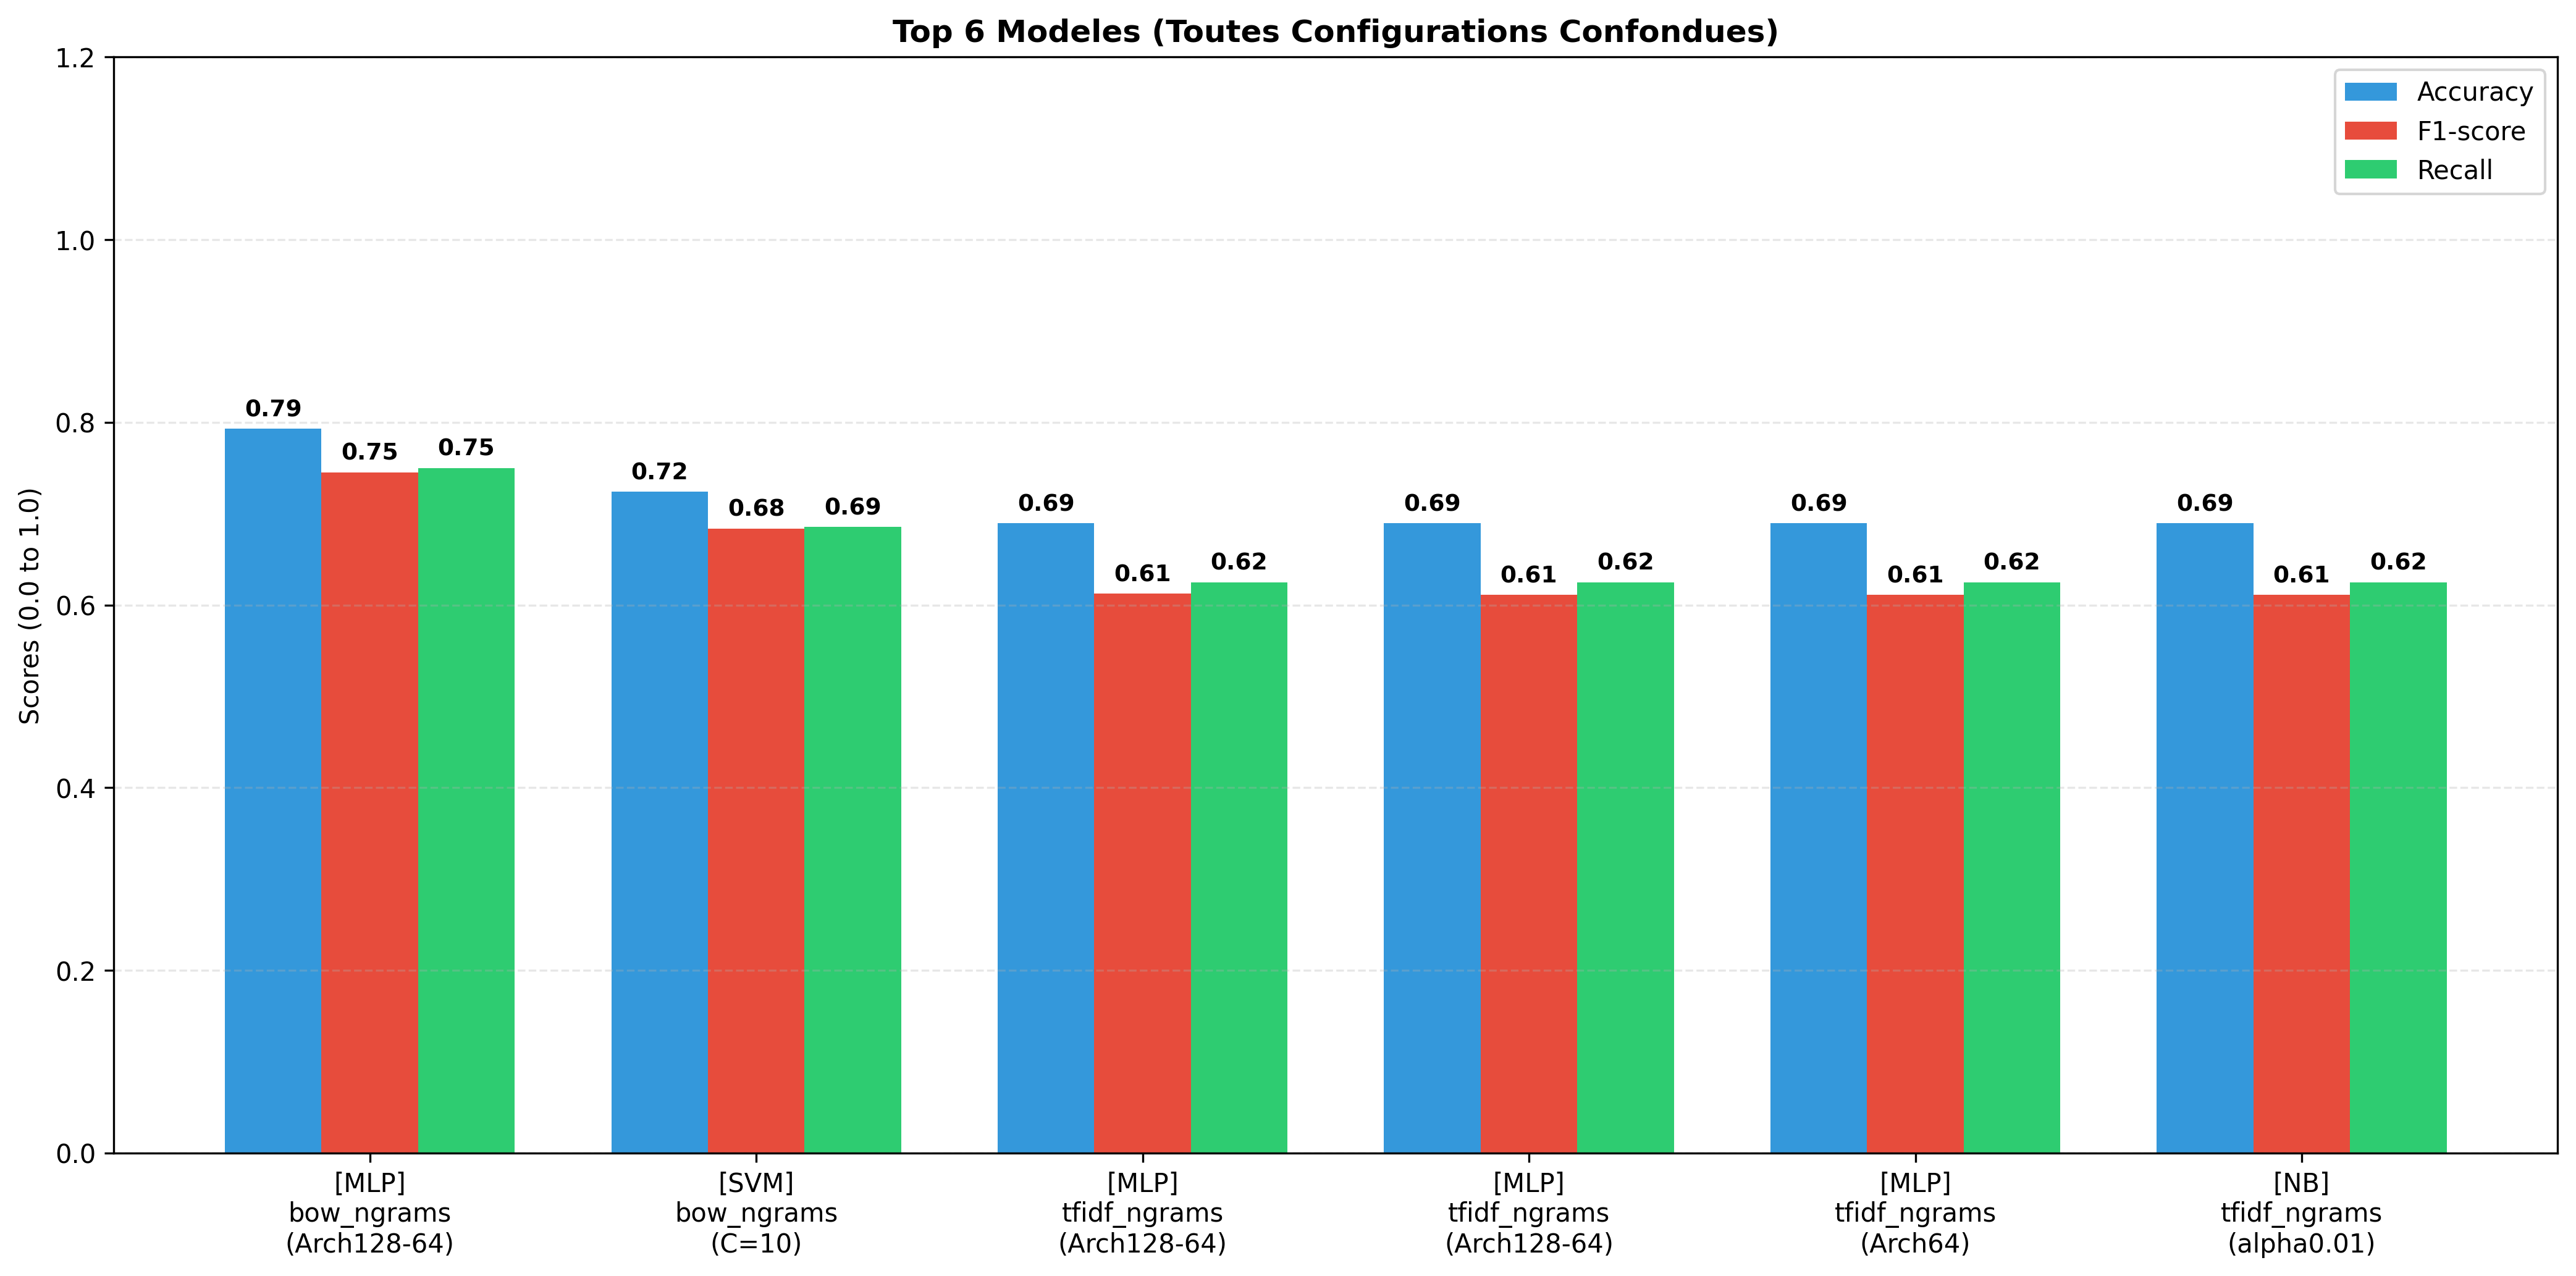
\includegraphics[width=\textwidth]{Top_6_Modeles_Toutes_Configurations_Confondues.png}
    \caption{Top 6 configurations toutes méthodes confondues}
    \label{fig:global}
\end{figure}

La Figure~\ref{fig:global} confirme que les meilleures performances sont entièrement dominées par le SVM. La configuration \textbf{SVM + TF-IDF N-grammes ($C=10$)} reste la meilleure de l'ensemble des 84 configurations testées avec un F1-score de 0,61.

\subsubsection{Comparaison globale par classifieur}

\begin{table}[H]
\centering
\caption{Meilleure configuration par classifieur}
\label{tab:synthese}
\begin{tabular}{lllccc}
\toprule
\textbf{Classifieur} & \textbf{Meilleure représentation} & \textbf{Paramètre} & \textbf{Acc.} & \textbf{F1} & \textbf{Recall} \\
\midrule
SVM    & tfidf\_ngrams & $C=10$           & \textbf{0,69} & \textbf{0,61} & \textbf{0,62} \\
CNB    & tfidf\_ngrams & $\alpha=0{,}01$  & \textbf{0,69} & \textbf{0,61} & \textbf{0,62} \\
$k$-NN & tfidf\_ngrams & $k=1$            & 0,59 & 0,57 & 0,59 \\
MLP    & tfidf         & LR=0,001, [64]   & $\sim$0,52 & $\sim$0,46 & $\sim$0,48 \\
\bottomrule
\end{tabular}
\end{table}

\subsection{Analyse des résultats}

\subsubsection{TF-IDF N-grammes : la représentation dominante}

Quelle que soit la méthode de classification, \textbf{TF-IDF N-grammes} se classe systématiquement dans le Top-2 des représentations. Deux facteurs cumulatifs expliquent ce résultat : la pondération TF-IDF filtre les termes trop fréquents et peu discriminants, et les trigrammes capturent des séquences de mots caractéristiques du plagiat de type \texttt{cut}, où des expressions entières sont reprises verbatim du texte source.

\subsubsection{Supériorité du SVM}

Le SVM avec noyau cosinus surpasse tous les autres classifieurs avec un écart notable sur le F1-score (0,61 contre 0,57 pour le $k$-NN). Cette supériorité est cohérente avec la littérature : le SVM est très efficace sur des données textuelles de haute dimension grâce à sa capacité à trouver des frontières de décision précises même dans des espaces sparses.

\subsubsection{Criticité de la régularisation SVM}

L'écart entre $C=10$ (F1=0,61) et $C=0,1$ (F1=0,14) est considérable. Avec un $C$ trop faible, la régularisation est trop forte et le modèle sous-apprend complètement. Sur un corpus de 95 documents, un $C$ élevé ($C=10$) est clairement préférable.

\subsubsection{Le $k$-NN préfère $k=1$}

La valeur $k=1$ est systématiquement la meilleure pour le $k$-NN. Cela indique que dans l'espace de représentation choisi, le document le plus proche est presque toujours de la même classe. Augmenter $k$ dilue cette information en incluant des voisins moins pertinents.

\subsubsection{Difficulté de la classe \texttt{light}}

Les performances globales (55--69\,\% d'accuracy sur 4 classes) sont raisonnables, mais la classe \texttt{light} (plagiat léger par substitution de synonymes) est probablement la source principale d'erreurs résiduelles. Les représentations lexicales ne peuvent pas détecter qu'un synonyme a remplacé un mot du texte source : les deux mots sont traités comme des features indépendantes. Ce problème nécessite des représentations sémantiques (word embeddings, BERT) pour être vraiment résolu.

\subsubsection{Limitation du MLP}

Avec seulement 66 documents d'entraînement, le MLP souffre d'un risque important de sur-apprentissage. L'architecture $[128, 64]$ est plus expressive mais plus difficile à entraîner sur si peu de données. L'architecture $[64]$ et un learning rate de 0,001 sont plus stables. Les performances restent inférieures au SVM, ce qui illustre que la profondeur d'un réseau de neurones est un avantage principalement visible avec de grandes quantités de données.

\section{Conclusion}

\subsection{Récapitulatif de la problématique et de la réalisation}

Ce projet avait pour objectif de construire un système automatique de détection du plagiat textuel capable de distinguer quatre niveaux : absence de plagiat (\texttt{non}), plagiat léger (\texttt{light}), plagiat lourd (\texttt{heavy}) et copie directe (\texttt{cut}). Le corpus utilisé, extrait du benchmark PAN, contient 95 documents avec un léger déséquilibre en faveur de la classe \texttt{non}.

Nous avons conçu et implémenté un pipeline modulaire complet comprenant six méthodes de représentation vectorielle et quatre classifieurs d'apprentissage automatique, dont un réseau de neurones MLP développé entièrement from scratch en NumPy. Au total, \textbf{84 configurations} ont été testées et évaluées selon trois métriques : accuracy, F1-score macro et recall macro.

\subsection{Récapitulatif des résultats}

\begin{itemize}
    \item La combinaison \textbf{SVM + TF-IDF N-grammes ($C=10$)} est la meilleure configuration (accuracy 0,69, F1-score 0,61, recall 0,62).
    \item La représentation \textbf{TF-IDF N-grammes} (trigrammes) est systématiquement supérieure au BoW simple.
    \item Le \textbf{SVM avec noyau cosinus} est le classifieur le plus performant, confirmé dans toutes les configurations.
    \item Le \textbf{$k$-NN avec $k=1$} est compétitif (F1=0,57) et constitue une alternative simple.
    \item Le \textbf{MLP from scratch} valide l'implémentation complète d'un réseau de neurones, mais ses performances restent limitées par la taille du corpus.
    \item La classe \textbf{\texttt{light}} reste la plus difficile à détecter avec des approches lexicales.
\end{itemize}

\vspace{1cm}
\noindent\rule{\linewidth}{0.5pt}
\vspace{0.3cm}

\begin{center}
\textit{Projet NLP --- Détection automatique du plagiat textuel ---}\\[4pt]
\textit{REZGUI Léna \quad|\quad SETTI Mohamed Chaib \quad|\quad BENSADI Aris \quad|\quad LAMAIRI Mohamed Yassine}\\[4pt]
\end{center}

\end{document}
